%!TEX TS-program = xelatex

% Шаблон документа LaTeX создан в 2018 году
% Алексеем Подчезерцевым
% В качестве исходных использованы шаблоны
% 	Данилом Фёдоровых (danil@fedorovykh.ru) 
%		https://www.writelatex.com/coursera/latex/5.2.2
%	LaTeX-шаблон для русской кандидатской диссертации и её автореферата.
%		https://github.com/AndreyAkinshin/Russian-Phd-LaTeX-Dissertation-Template

\documentclass[a4paper,14pt]{article}


%%% Работа с русским языком
\usepackage[english,russian]{babel}   %% загружает пакет многоязыковой вёрстки
\usepackage{fontspec}      %% подготавливает загрузку шрифтов Open Type, True Type и др.
\defaultfontfeatures{Ligatures={TeX},Renderer=Basic}  %% свойства шрифтов по умолчанию
\setmainfont[Ligatures={TeX,Historic}]{Times New Roman} %% задаёт основной шрифт документа
\setsansfont{Comic Sans MS}                    %% задаёт шрифт без засечек
\setmonofont{Courier New}
\usepackage{indentfirst}
\frenchspacing

\renewcommand{\epsilon}{\ensuremath{\varepsilon}}
\renewcommand{\phi}{\ensuremath{\varphi}}
\renewcommand{\kappa}{\ensuremath{\varkappa}}
\renewcommand{\le}{\ensuremath{\leqslant}}
\renewcommand{\leq}{\ensuremath{\leqslant}}
\renewcommand{\ge}{\ensuremath{\geqslant}}
\renewcommand{\geq}{\ensuremath{\geqslant}}
\renewcommand{\emptyset}{\varnothing}

%%% Дополнительная работа с математикой
\usepackage{amsmath,amsfonts,amssymb,amsthm,mathtools} % AMS
\usepackage{icomma} % "Умная" запятая: $0,2$ --- число, $0, 2$ --- перечисление

%% Номера формул
%\mathtoolsset{showonlyrefs=true} % Показывать номера только у тех формул, на которые есть \eqref{} в тексте.
%\usepackage{leqno} % Нумерация формул слева	

%% Перенос знаков в формулах (по Львовскому)
\newcommand*{\hm}[1]{#1\nobreak\discretionary{}
	{\hbox{$\mathsurround=0pt #1$}}{}}

%%% Работа с картинками
\usepackage{graphicx}  % Для вставки рисунков
\graphicspath{{images/}}  % папки с картинками
\setlength\fboxsep{3pt} % Отступ рамки \fbox{} от рисунка
\setlength\fboxrule{1pt} % Толщина линий рамки \fbox{}
\usepackage{wrapfig} % Обтекание рисунков текстом

%%% Работа с таблицами
\usepackage{array,tabularx,tabulary,booktabs} % Дополнительная работа с таблицами
\usepackage{longtable}  % Длинные таблицы
\usepackage{multirow} % Слияние строк в таблице
\usepackage{float}% http://ctan.org/pkg/float

%%% Программирование
\usepackage{etoolbox} % логические операторы


%%% Страница
\usepackage{extsizes} % Возможность сделать 14-й шрифт
\usepackage{geometry} % Простой способ задавать поля
\geometry{top=20mm}
\geometry{bottom=20mm}
\geometry{left=20mm}
\geometry{right=10mm}
%
%\usepackage{fancyhdr} % Колонтитулы
% 	\pagestyle{fancy}
%\renewcommand{\headrulewidth}{0pt}  % Толщина линейки, отчеркивающей верхний колонтитул
% 	\lfoot{Нижний левый}
% 	\rfoot{Нижний правый}
% 	\rhead{Верхний правый}
% 	\chead{Верхний в центре}
% 	\lhead{Верхний левый}
%	\cfoot{Нижний в центре} % По умолчанию здесь номер страницы

\usepackage{setspace} % Интерлиньяж
\onehalfspacing % Интерлиньяж 1.5
%\doublespacing % Интерлиньяж 2
%\singlespacing % Интерлиньяж 1

\usepackage{lastpage} % Узнать, сколько всего страниц в документе.

\usepackage{soul} % Модификаторы начертания

\usepackage{hyperref}
\usepackage[usenames,dvipsnames,svgnames,table,rgb]{xcolor}
\hypersetup{				% Гиперссылки
	unicode=true,           % русские буквы в раздела PDF
	pdftitle={Заголовок},   % Заголовок
	pdfauthor={Автор},      % Автор
	pdfsubject={Тема},      % Тема
	pdfcreator={Создатель}, % Создатель
	pdfproducer={Производитель}, % Производитель
	pdfkeywords={keyword1} {key2} {key3}, % Ключевые слова
	colorlinks=true,       	% false: ссылки в рамках; true: цветные ссылки
	linkcolor=black,          % внутренние ссылки
	citecolor=black,        % на библиографию
	filecolor=magenta,      % на файлы
	urlcolor=black           % на URL
}
\makeatletter 
\def\@biblabel#1{#1. } 
\makeatother
\usepackage{cite} % Работа с библиографией
%\usepackage[superscript]{cite} % Ссылки в верхних индексах
%\usepackage[nocompress]{cite} % 
\usepackage{csquotes} % Еще инструменты для ссылок

\usepackage{multicol} % Несколько колонок

\usepackage{tikz} % Работа с графикой
\usepackage{pgfplots}
\usepackage{pgfplotstable}

% ГОСТ заголовки
\usepackage[font=small]{caption}
%\captionsetup[table]{justification=centering, labelsep = newline} % Таблицы по правобу краю
%\captionsetup[figure]{justification=centering} % Картинки по центру


\newcommand{\tablecaption}[1]{\addtocounter{table}{1}\small \begin{flushright}\tablename \ \thetable\end{flushright}%	
\begin{center}#1\end{center}}

\newcommand{\imref}[1]{рис.~\ref{#1}}

\usepackage{multirow}
\usepackage{spreadtab}
\newcolumntype{K}[1]{@{}>{\centering\arraybackslash}p{#1cm}@{}}


\usepackage{xparse}
\usepackage{fancyvrb}

\RecustomVerbatimCommand{\VerbatimInput}{VerbatimInput}
{
	fontsize=\footnotesize    
}

\usepackage{tocloft}
\renewcommand{\cftsecleader}{\cftdotfill{\cftdotsep}}
\begin{document} % конец преамбулы, начало документа
	\begin{titlepage}
	\begin{center}
 		ФЕДЕРАЛЬНОЕ  ГОСУДАРСТВЕННОЕ АВТОНОМНОЕ \\
		ОБРАЗОВАТЕЛЬНОЕ УЧРЕЖДЕНИЕ ВЫСШЕГО ОБРАЗОВАНИЯ\\
		«НАЦИОНАЛЬНЫЙ ИССЛЕДОВАТЕЛЬСКИЙ УНИВЕРСИТЕТ\\
		«ВЫСШАЯ ШКОЛА ЭКОНОМИКИ»
	\end{center}
	
	\begin{center}
		\textbf{Московский институт электроники и математики}
		
		\textbf{им. А.Н.Тихонова НИУ ВШЭ}
		
		\vspace{2ex}
		
		\textbf{Департамент компьютерной инженерии}
	\end{center}
	\vspace{1ex}	
	
	\begin{center}
	\textbf{ОТЧЕТ\\
		ПО ЛАБОРАТОРНОЙ РАБОТЕ №6
	}
	\end{center}	
	\vspace{2ex}
	\begin{center}
		по дисциплине «Проектирование систем на кристалле»
	\end{center}	

	\vspace{2ex}

	\begin{flushright}
		\textbf{Выполнили:}
		
		\vspace{2ex}
		
		Студенты группы БИВ174
		
		Бригада №5
		
		\vspace{2ex}
		
		Подчезерцев Алексей Евгеньевич
		
		Солодянкин Андрей Александрович
		\vspace{2ex}
		
	\end{flushright}

	\vfill
	\begin{center}
		Москва \the\year \, г.
	\end{center}
	
\end{titlepage}
\addtocounter{page}{1}
	\tableofcontents
	\pagebreak
	\section{Задание}
	
	\begin{enumerate}
		\item Увеличьте разрядность данных до 8, а количество ячеек до 2048. Представьте результаты
		моделирования и синтеза в RTL и объясните их. Загрузите результаты в Technology Мар
		Viewer и дайте описание того, что получится.
		
		\item Самостоятельно изучите решение описанной выше проблемы (например, в обсуждении на
		форуме Electronix). Реализовать ПЗУ на встроенной памяти.
		
		\item Измените целевую микросхему на любой чип из семейства Cyclone V. Представьте
		результаты компиляции и синтеза в RTL и объясните их. Загрузите результаты в Technology
		Мар Viewer и опишите полученные результаты.
		
		\item Проверьте , как изменится размер двухпортовой памяти при увеличении разрядности шины
		адреса до 8, 10, 12, 16 бит. Представьте результаты компиляции и синтеза в RTL, опишите и
		объясните полученные результаты.
		
		\item Проанализируйте, как изменится размер стека при увеличении глубины стека до 32, 64, 128,
		256 элементов. Представьте результаты компиляции и синтеза в RTL Viewer и объясните их.
		Загрузите результаты в Technology Мар Viewer, опишите и объясните полученные
		результаты.
		
		\item Реализуйте два варианта очереди как в случае со стеком в Разделе 7.9 с глубиной до 32, 64,
		128, 256 элементов. Представьте результаты компиляции и синтеза в RTL Viewer и объясните
		их. Загрузите результаты в Technology Мар Viewer, опишите и объясните полученные
		результаты.
		
		\item Модифицируйте пример и з Листинга 7.16 так, чтобы данный модуль был
		параметризируемый, и можно было задать память любого размера кратного 16 словам по 6
		бит. Опишите полученный модуль и его работу.
	\end{enumerate}
	
	\section{Дополнительные задания}
	
	\subsection{Задание 1}
	
	На RTL представлении можно видеть 2 блока: первый это синхронный D-триггер в который записывается текущий адрес, второй блок представлен блолом RAM. На TMV можно видеть 8 синхронный однобитных D-триггеров, в которых хранится текущий адрес. Информация хранится в 8 блоках RAM по 256 бит каждый.
	
	RLT диаграмма на рис. \ref{fig:z1_rtl}. Technology Мар Viewer на рис. \ref{fig:z1_tmv}.
	 
	\begin{figure}[H]
		\centering
		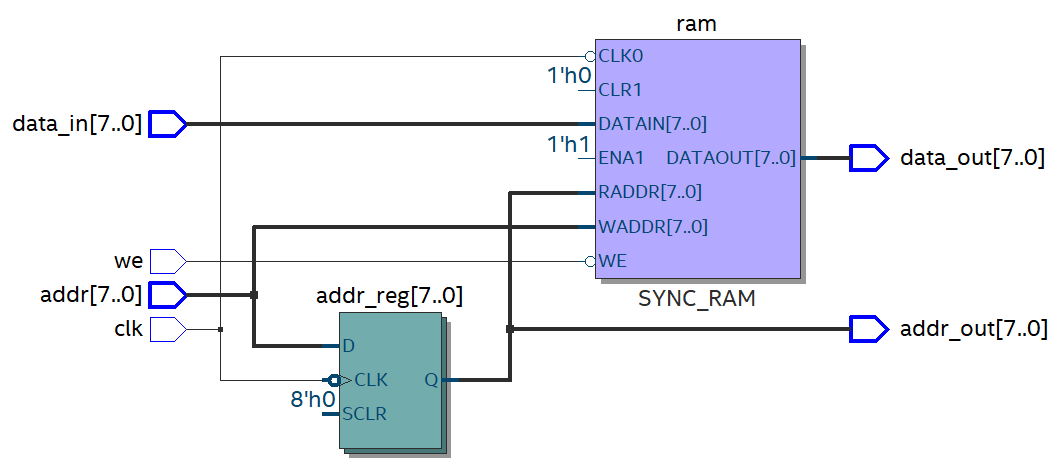
\includegraphics[width=\linewidth]{images/z1_rtl}
		\caption{RTL-схема}
		\label{fig:z1_rtl}
	\end{figure}

	\begin{figure}[H]
		\centering
		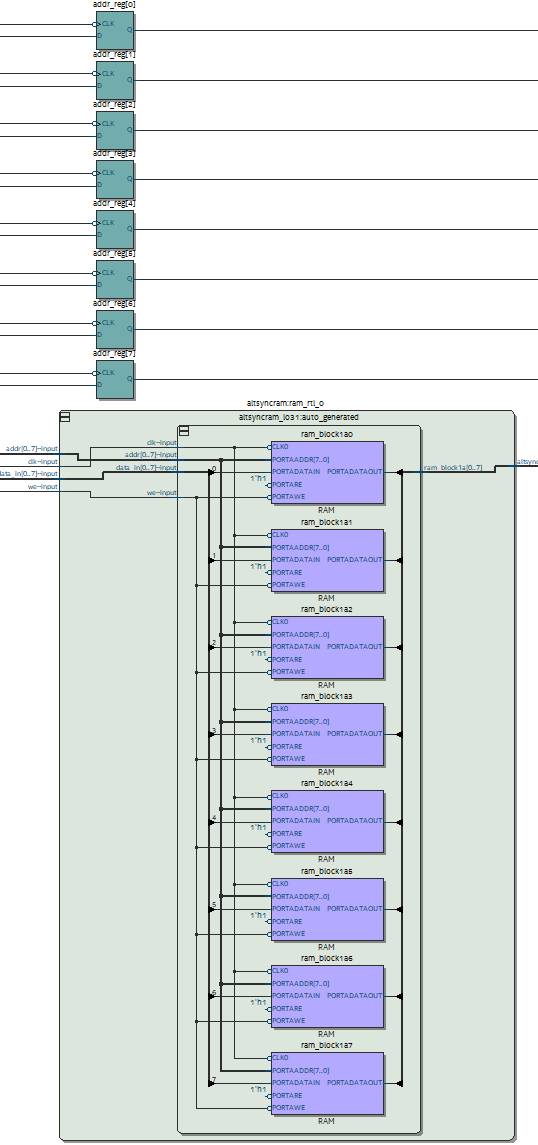
\includegraphics[width=0.65\linewidth]{images/z1_tmv}
		\caption{Technology Мар Viewer}
		\label{fig:z1_tmv}
	\end{figure}

	\VerbatimInput{../z1/lab7_3.v}
	
	
	\section{Задания для самостоятельной работы}
	
	Разработайте схему простой двухпортовой памяти, которая будет хранить данные о
	цветном изображении с глубиной цвета 8 бит и разрешением 212х104.
			
	\section{Контрольные вопросы}
	
	\begin{enumerate}
		\item Опишите, как строятся регистры на основе D-триггеров.
		
		\item Как организованы массивы ячеек памяти?
		
		\item Приведите примеры типов входов и выходов памяти. Опишите их назначение.
		
		\item Какими бывают режимы работы памяти? Опишите их.
		
		\item Какими бывают виды двухпортовой памяти? Опишите режимы ее работы.
		
		\item Что такое «информационная емкость»? Как ее рассчитать?
		
		\item Какими бывают типы запоминающих устройств?
		
		\item Как можно классифицировать память по функциям, которые она выполняет?
		
		\item Как устроен логический элемент микросхемы lntel FPGA MAXl0?
		
		\item Опишите варианты конфигурации блока памяти М9К в микросхеме MAXl0.
		
		\item Как реализовать ПЗУ с помощью таблицы перекодировки? Приведите пример на Verilog.
		
		\item Для чего используется память вида «стек»? Опишите работу стека.
		
		\item Как реализовать стек с помощью сдвигового регистра? Приведите пример на Verilog.
		
		\item Как реализовать стек с помощью сдвига указателя? Приведите пример на Verilog.
		
		\item Как реализовать FIFO? Приведите пример на Verilog.
		
		\item Как устроена встроенная память микросхем ASIC?
	\end{enumerate}
	
	\section{Выводы по работе}
	
	В ходе работы получен опыт проектирования схем в программе Quartus с помощью языка Verilog.
	Полученное устройство было протестировано с помощью бенчтестов в программе Quartus Simulation Waveform editor и ModelSim.
	В процессе работы были смоделированы запоминающие устройства, очередь, стек.
	%В процессе работы были смоделированы различные шифраторы и дешифраторы, протестированы способы оптимизации схемы, а так же рассчитаны временные параметры схемы с различными способами оптимизации.
	В процессе был получен опыт работы с платой DE10-Lite, на которой проверялась работоспособность полученного устройства.
	
	\newpage 
	\renewcommand{\refname}{{\normalsize Список использованных источников}} 
	\centering 
	\begin{thebibliography}{9} 
		\addcontentsline{toc}{section}{\refname} 
		\bibitem{Verilog} Thomas D., Moorby P. The Verilog Hardware Description Language. – Springer Science \& Business Media, 2008.
		\bibitem{citekey} Khor W. Y. et al. Evaluation of FPGA Based QSPI Flash Access Using Partial Reconfiguration //2019 7th International Conference on Smart Computing \& Communications (ICSCC). – IEEE, 2019. – С. 1-5
	\end{thebibliography}
	
\end{document} % конец документа
